En gardant nos contraintes et enjeux en tête, il fallait trouver une façon efficace d'entraîner un modèle dans un temps raisonnable. Plusieurs techniques d'échantillonnage ont pu être testées.


\subsection{Échantillonnage fixe par classe}

Le premier modèle testé est un modèle pré-entraîné avec architecture \emph{Resnet18}, mais avec un seul canal de couleur au lieu de 3. Pour entraîner le modèle, on procède d'une manière alternative étant donné qu'on ne peut pas se permettre de faire de vraies epochs complètes. 



Ainsi, à chacune de nos "epochs", on échantillonne (sans remise) un nombre fixe $N$ de données par classe parmi nos 150 000 données par classe. Ces $340N$ données servent à faire une "epoch"  pour notre modèle. On procède de la même façon à chaque "epoch" en ré-échantillonnant dans nos 150 000 données par classe (même celles pigées aux anciennes "epochs"). 
En entraînant notre modèle de cette façon, il est possible que certaines données ne soient jamais vues et que d'autres le soient plusieurs fois.


Cette technique d'échantillonnage s'apparente au \emph{bootstrapping} utilisé pour les méthodes par ensemble. Elle agit à la fois comme méthode d'échantillonnage aléatoire et comme méthode de régularisation. 
On peut s'attendre à ce que le modèle n'overfit pas excessivement notre jeu de données d'entraînement en procédant de cette façon puisque les données ne seront pas vues plusieurs fois de façon rapide et le réseau ne peut donc pas les apprendre par coeur.


Si on fait 35 epochs de la sorte avec un nombre $N=500$ (epoch de 170 000 données) on peut voir approximativement 11\% des données totales et environ 5.45\% des données vues sont échantillonnées plus d'une fois parmi les 35 epochs. 
On peut voir qu'on est assez loin de voir la totalité du jeu de données même après les 35 epochs passées à cause de la quantité énorme de données disponibles. 
Toutefois, le modèle semble tout de même converger vers une précision de validation d'environ 76\% comme on peut le voir sur la figure \ref{histmodelnormal}. 
En utilisant un \emph{early stopping} et en utilisant les performances maximales sur le jeu de validation, on obtient une précision de validation de 77.44\%.


\begin{figure}[h]
	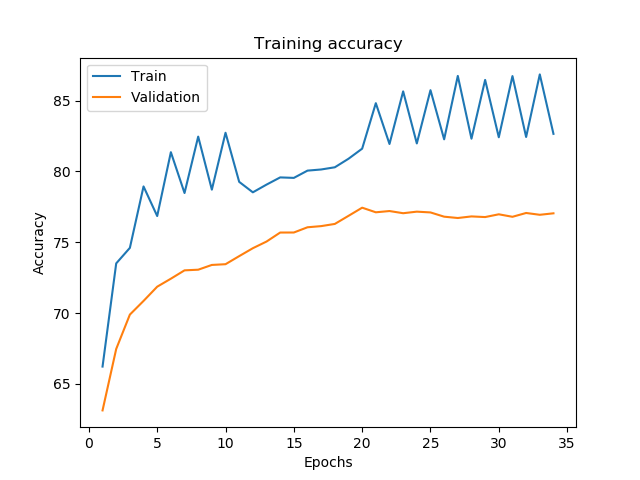
\includegraphics[width=\linewidth]{images/Model_general.png} % Figure image
	\caption{Historique d'entraînement avec entraînement standard} % Figure caption
	\label{histmodelnormal} 
\end{figure}


\subsection{Échantillonnage variable par classe}
La deuxième méthode d'entraînement est similaire à la première avec une légère modification qui essaie de privilégier les classes qui performent moins bien dans le but de simuler un processus de \emph{boosting}.


L'idée de base est d'échantillonner un plus grand nombre de données des classes qui sont mal prédites et un plus petit nombre pour celles qui sont bien prédites durant l'entraînement. 
À chaque epoch, on calcule notre précision par classe $A_i$ pour chacune des 340 classes. 
Pour effectuer notre epoch, on échantillonne $N_i$ données pour la classe i:

$$N_i=N(1-A_i)+0.25N$$
Où:
\begin{description}
\item[N]: Valeur constante pour toutes les classes (ex: 500)
\end{description}

Le terme $+0.25N$ permet de sélectionner au moins un minimum de données d'une classe qui performe déjà très bien pour que le modèle ne l'oublie pas lors la prochaine epoch.  Par exemple, on sélectionnerait $N$ données d'une classe avec 25\% de précision et $0.35N$ données d'une classe qui a 90\% de précision.


En appliquant cette technique d'apprentissage, on obtient une précision en validation de 79.53\% avec de l'early stopping. 
Cette technique d'échantillonnage ciblé nous permet d'aller chercher une précision supplémentaires d'environ 2\%.


\subsection{Modèle par ensemble avec couche de classification}
Le troisième modèle consiste à concaténer les sorties des 2 premiers modèles et à les passer dans une couche de classification linéaire. Pour l'entraînement de ce modèle, on gèle tous les paramètres des modèles \emph{Resnet18} et on entraîne seulement la couche de classification avec un échantillonnage fixe. La figure \ref{strutureensemble} illustre le processus.

\begin{figure}[h]
	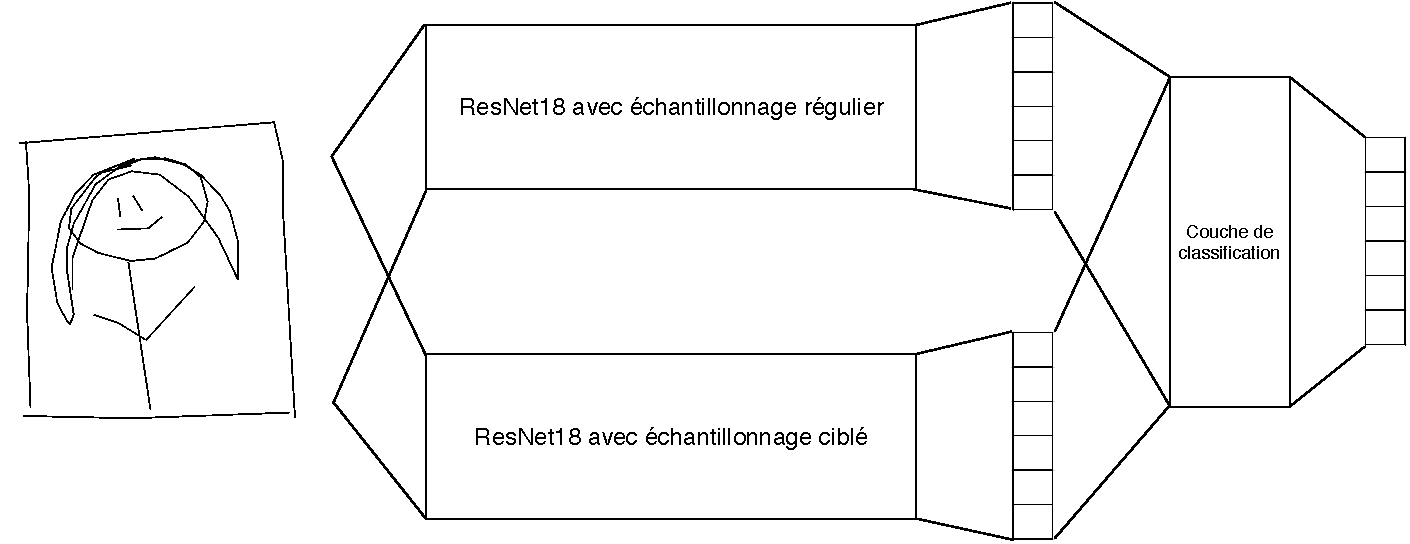
\includegraphics[width=\linewidth]{images/structure_reseau.pdf} % Figure image
	\caption{Modèle par ensemble avec couche de classification} % Figure caption
	\label{strutureensemble} 
\end{figure}


Par manque de temps, l'entraînement du modèle n'a pas pu être complété à 100\%, on peut toutefois voir l'historique d'entraînement du modèle sur la figure \ref{histmodelensemble}.


\begin{figure}[h]
	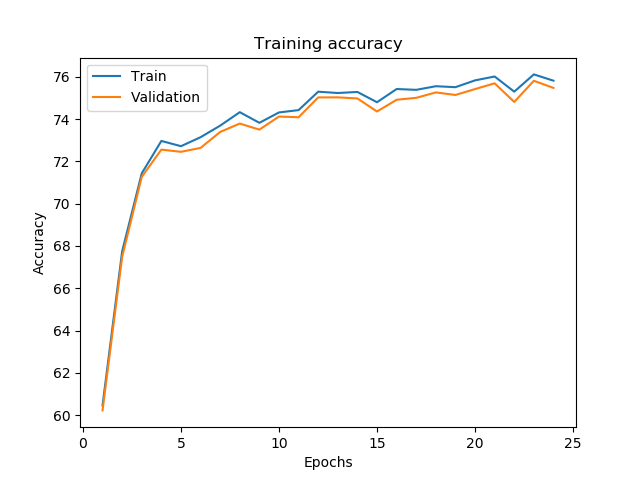
\includegraphics[width=\linewidth]{images/Model_ensemble.png} % Figure image
	\caption{Historique d'entraînement} % Figure caption
	\label{histmodelensemble} 
\end{figure}


On voit que la précision sur le jeu d'entraînement est pratiquement identique à celle de validation et qu'elles ne semblent pas encore avoir atteint un plateau lors de l'entraînement que nous avons fait. Il aurait été intéressant de voir les résultats après convergence puisque nous pensons que cette technique aurait pu nous permettre d'obtenir des performances légèrement supérieures à notre deuxième modèle. 
Avec un \emph{early stopping}, on obtient une précision de 75.81\% en validation. 


\subsection{Modèle par ensemble avec moyenne simple des 2 premiers modèles}

Le dernier modèle que nous avons essayé est simplement d'utiliser la prédiction moyenne faite selon nos deux modèles \emph{ResNet18}. 
Cette technique par ensemble nous permet d'obtenir une précision de 79.94\% en validation, ce qui est légèrement supérieur à notre deuxième modèle entraîné avec échantillonnage ciblé. 

